% ============================================================
% Companion slides for the course
%   Python for AI-Driven Automation and Business Data Science
%
% Style: Madrid theme with horizontal section navigation bar
% Language: English
% Compile with:  pdflatex course_slides.tex   (run twice)
% ============================================================

\documentclass[aspectratio=169,11pt]{beamer}

% ---- Encoding & language -----------------------------------
\usepackage[utf8]{inputenc}
\usepackage[T1]{fontenc}
\usepackage{lmodern}                % Latin Modern fonts (no missing-font errors)
\usepackage[english]{babel}

% ---- Core packages -----------------------------------------
\usepackage{graphicx}
\usepackage{booktabs}
\usepackage{amsmath,amssymb,amsfonts}
\usepackage{mathtools}
\usepackage{hyperref}
\usepackage{xcolor}
\usepackage{verbatim}
\usepackage{alltt}
\usepackage{tikz}

% ---- Beamer theme ------------------------------------------
\usetheme{Madrid}
\usecolortheme{default}
\setbeamertemplate{navigation symbols}{}
\setbeamertemplate{footline}[frame number]
\setbeamertemplate{blocks}[rounded][shadow=false]

% ---- Section navigation bar in headline --------------------
\setbeamertemplate{headline}{%
  \leavevmode%
  \hbox{%
    \begin{beamercolorbox}[wd=\paperwidth,ht=2.5ex,dp=1.125ex]{section in head/foot}%
      \insertsectionnavigationhorizontal{\paperwidth}{}{\hskip0pt plus1filll}%
    \end{beamercolorbox}%
  }%
}

% ---- Code listings -----------------------------------------
\usepackage{listings}
\definecolor{codebg}{HTML}{F6F8FA}
\definecolor{codegreen}{HTML}{55A467}
\definecolor{codeblue}{HTML}{4C72B0}
\definecolor{codegray}{HTML}{7F7F7F}

\lstdefinestyle{Pystyle}{
  language=Python,
  basicstyle=\ttfamily\footnotesize,
  keywordstyle=\color{codeblue}\bfseries,
  commentstyle=\color{codegray}\itshape,
  stringstyle=\color{codegreen},
  showstringspaces=false,
  numbers=none,
  backgroundcolor=\color{codebg},
  frame=single,
  rulecolor=\color{codegray!50},
  columns=fullflexible,
  upquote=true,
  breaklines=true,
  literate={→}{$\rightarrow$}{1}
           {≥}{$\geq$}{1}
           {≤}{$\leq$}{1}
           {²}{${}^2$}{1}
           {π}{$\pi$}{1}
}
\lstset{style=Pystyle}

% ---- Auto section overview slides --------------------------
\AtBeginSection[]{%
  \begin{frame}{Outline}
    \tableofcontents[currentsection,sectionstyle=show/shaded,subsectionstyle=show/show/hide]
  \end{frame}
}

% ============================================================
% TITLE BLOCK
% ============================================================
\title{Python for AI-Driven Automation\\and Business Data Science}
\subtitle{Companion slides to the 11-notebook course}
\author{Course materials}
\institute{}
\date{}


% ============================================================
\begin{document}
% ============================================================

% ---- Title slide -------------------------------------------
\begin{frame}
  \titlepage
\end{frame}

% ---- Table of contents -------------------------------------
\begin{frame}{Contents}
  \tableofcontents[hideallsubsections]
\end{frame}


% ============================================================
\section{Overview}
% ============================================================

\subsection{The course in one diagram}

\begin{frame}{What you will learn}
  \begin{center}
    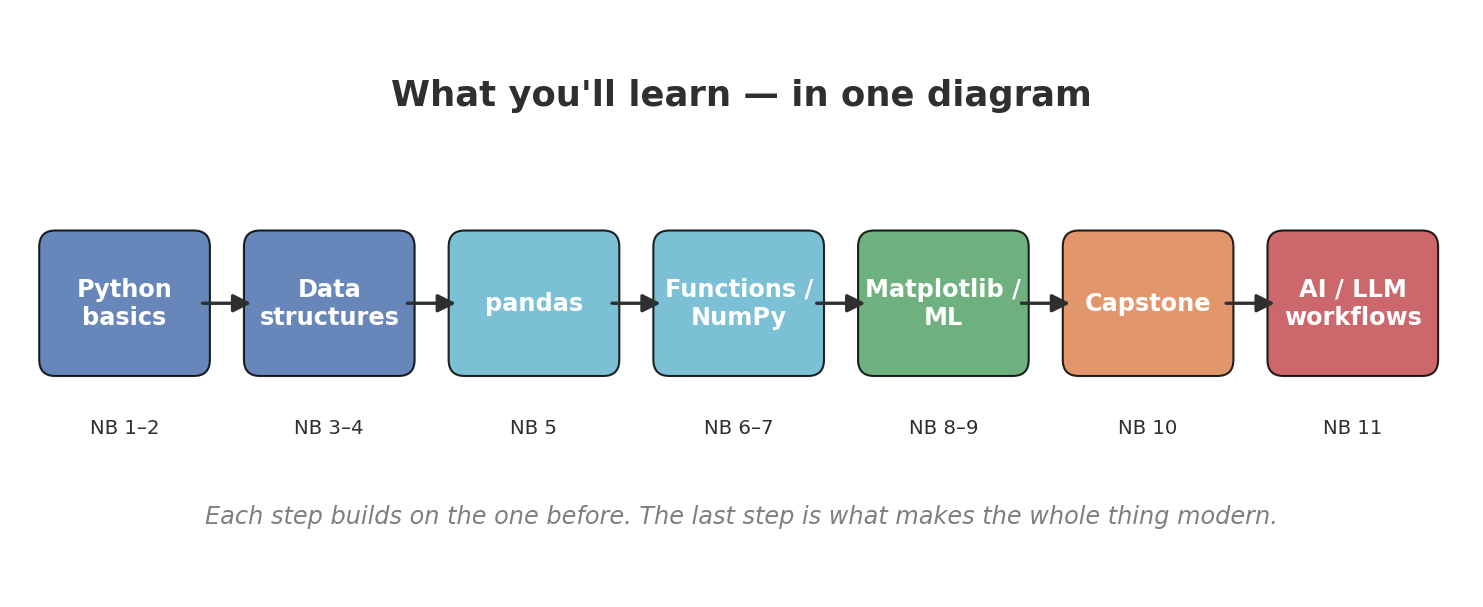
\includegraphics[width=0.97\textwidth,height=0.78\textheight,keepaspectratio]{images/01_course_arc.png}
  \end{center}
\end{frame}

\subsection{Why this course}

\begin{frame}{Why this course exists}
  \begin{block}{The 2015 way of teaching Python}
    Print statements, fizz-buzz, a quick tour of pandas, maybe a linear
    regression at the end.
  \end{block}
  \vspace{4pt}
  \begin{exampleblock}{What working with data actually looks like in 2025}
    \begin{itemize}
      \item Calling APIs, parsing JSON, retrying on failure.
      \item Cleaning messy text, building dashboards, training small models.
      \item Calling an LLM as a function -- and getting structured output back.
    \end{itemize}
  \end{exampleblock}
  \vspace{4pt}
  This course teaches Python through the second lens from the very first cell.
\end{frame}

\begin{frame}{Three skills the modern data role asks for}
  \begin{enumerate}
    \item \textbf{Solid Python fluency} -- reading and writing code without friction.
    \item \textbf{Working with data professionally} -- cleaning, exploring, modelling, visualising.
    \item \textbf{AI-driven automation} -- using LLMs, APIs, and small scripts to replace repetitive analytical work.
  \end{enumerate}
  \vspace{8pt}
  All three are exercised across the 11 notebooks.
\end{frame}

\begin{frame}{Course at a glance}
  \small
  \begin{tabular}{lll}
    \toprule
    \textbf{NB} & \textbf{Topic} & \textbf{What you build} \\
    \midrule
    1  & Python basics              & A KPI snapshot for an AI support bot \\
    2  & Control structures         & A ticket-triage rules engine \\
    3  & Lists \& sequences         & Latency-log analysis \\
    4  & Dictionaries / JSON        & A defensive API-response parser \\
    5  & Pandas preview             & LLM-call log analysis \\
    6  & Functions \& modules       & A reusable cost / clean toolkit \\
    7  & NumPy fundamentals         & A/B-testing two LLM providers \\
    8  & Matplotlib basics          & A 2$\times$2 AI-ops dashboard \\
    9  & scikit-learn               & Customer-churn prediction \\
    10 & Capstone                   & End-to-end AI support analytics \\
    11 & AI-assisted workflows      & LLM prompts, RAG, automation \\
    \bottomrule
  \end{tabular}
\end{frame}


% ============================================================
\section{Python Fundamentals}
% ============================================================

\subsection{Variables and types}

\begin{frame}[fragile]{Variables -- labels on values}
  \begin{exampleblock}{From an AI-automation project}
\begin{lstlisting}
model_name     = "gpt-4o-mini"   # which model
price_per_1k   = 0.0006           # USD per 1K input tokens
monthly_tokens = 14_500_000       # expected volume
is_production  = True
\end{lstlisting}
  \end{exampleblock}
  \begin{itemize}
    \item Five core types you meet daily: \texttt{int}, \texttt{float}, \texttt{str}, \texttt{bool}, \texttt{None}.
    \item \texttt{snake\_case} names that mean something to a stranger.
    \item Underscores in numbers (\texttt{14\_500\_000}) just for readability.
  \end{itemize}
\end{frame}

\begin{frame}[fragile]{Strings arrive from APIs -- and they look like numbers}
  \begin{alertblock}{The most common parsing bug}
    \texttt{"25" + 5} raises \texttt{TypeError}: you cannot add a string to an int.
  \end{alertblock}
\begin{lstlisting}
raw_tokens = "1024"             # comes back as a string
tokens     = int(raw_tokens)     # convert before doing maths

int(3.9)   # 3  -- truncates toward zero, does NOT round
round(3.9) # 4
\end{lstlisting}
  Convert with \texttt{int()}, \texttt{float()}, \texttt{str()}, \texttt{bool()} -- the bread and butter of cleaning real data.
\end{frame}

\subsection{Arithmetic for AI workloads}

\begin{frame}[fragile]{Costing a batch of LLM calls in 4 lines}
\begin{lstlisting}
n_tickets        = 350
tokens_per_call  = 600
price_per_1k_tok = 0.0006

total_cost = n_tickets * tokens_per_call / 1000 * price_per_1k_tok
print(f"Total cost: ${total_cost:.4f}")    # Total cost: $0.1260
\end{lstlisting}
  \begin{block}{The pattern that scales}
    \emph{Inputs at the top} $\rightarrow$ \emph{derived values} $\rightarrow$ \emph{readable output}.
    Edit one input, re-run, done.
  \end{block}
\end{frame}

\begin{frame}{Token cost scales fast}
  \begin{center}
    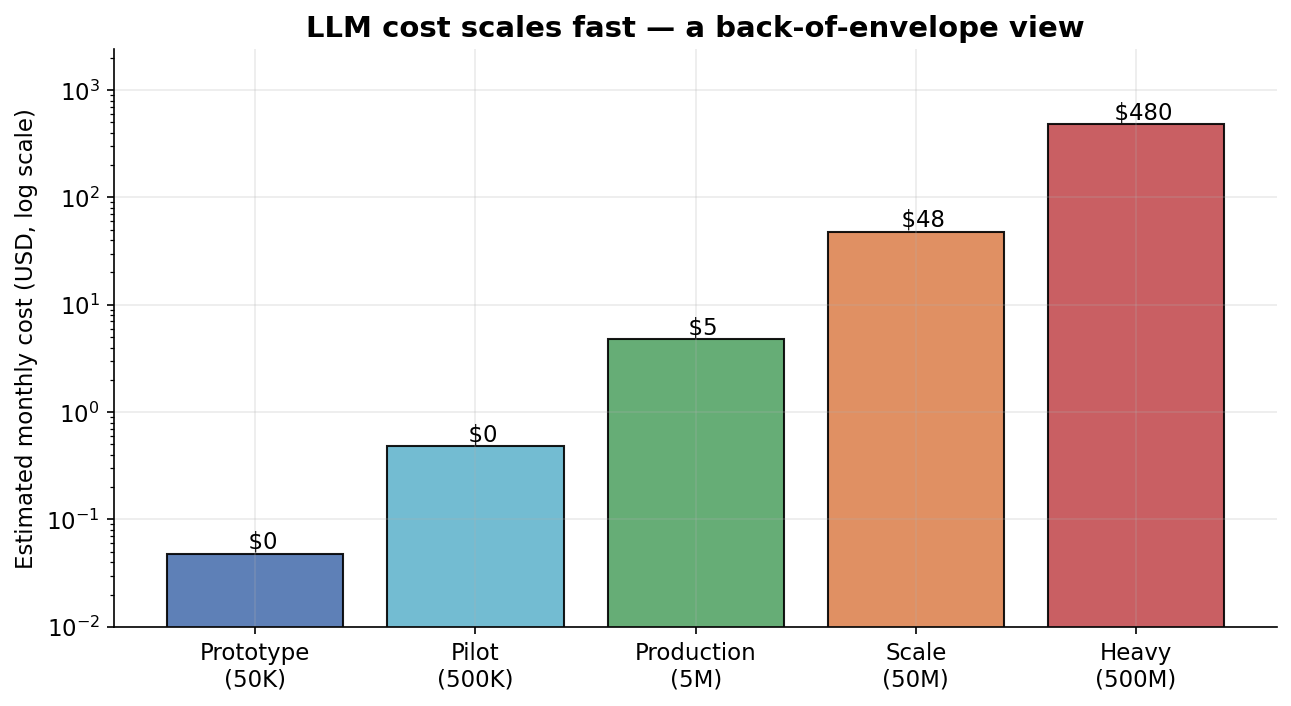
\includegraphics[width=0.95\textwidth,height=0.75\textheight,keepaspectratio]{images/02_token_cost_scenarios.png}
  \end{center}
\end{frame}

\subsection{Decisions and loops}

\begin{frame}{A rules engine for ticket triage}
  \begin{center}
    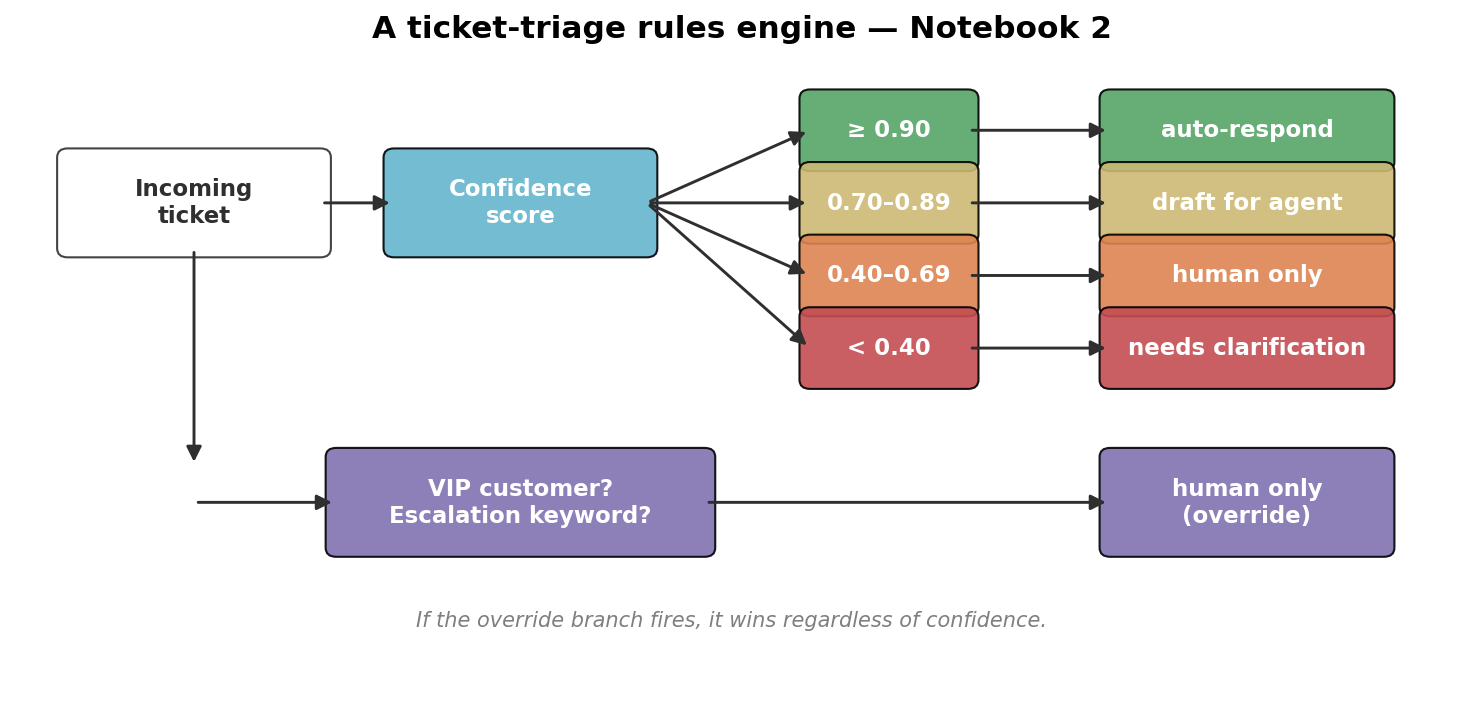
\includegraphics[width=\textwidth,height=0.78\textheight,keepaspectratio]{images/03_triage_rules.png}
  \end{center}
\end{frame}

\begin{frame}[fragile]{The same engine in Python}
\begin{lstlisting}
def route_ticket(confidence, is_vip, message):
    text = message.lower()
    if any(w in text for w in ("urgent", "escalate", "refund")):
        return "human-only"
    if is_vip and confidence < 0.8:
        return "human-only"
    if confidence >= 0.90: return "auto-respond"
    if confidence >= 0.70: return "draft-for-agent"
    if confidence >= 0.40: return "human-only"
    return "needs-clarification"
\end{lstlisting}
  \begin{alertblock}{Branch order matters}
    Most restrictive condition first. Otherwise enterprise customers
    fall into the SMB tier.
  \end{alertblock}
\end{frame}

\begin{frame}[fragile]{Retry-with-backoff -- the \texttt{while} pattern}
\begin{lstlisting}
attempt, success = 0, False
while attempt < max_attempts and not success:
    attempt += 1
    success = call_api()
    if not success:
        wait = 0.5 * 2 ** (attempt - 1)  # exponential backoff
        time.sleep(wait)
\end{lstlisting}
  \begin{block}{Two stop conditions joined by \texttt{and}}
    \emph{Keep trying while I haven't succeeded \textbf{and} I haven't burned
    through my budget.}
    The safest shape for any retry loop.
  \end{block}
\end{frame}

\subsection{Functions}

\begin{frame}[fragile]{Wrap reusable logic behind a name}
\begin{lstlisting}
def call_cost(tokens_in, tokens_out,
              price_in_per_1k=0.0006,
              price_out_per_1k=0.0024) -> float:
    """USD cost of one LLM call from token usage."""
    return (tokens_in  / 1000 * price_in_per_1k +
            tokens_out / 1000 * price_out_per_1k)

call_cost(800, 200)              # $0.000960
call_cost(800, 200, 0.0010)      # $0.001280  -- override one default
\end{lstlisting}
  \begin{block}{Four wins you get for free}
    A meaningful \emph{name}, \emph{testability}, \emph{reusability}, \emph{one place to change} when the price moves.
  \end{block}
\end{frame}


% ============================================================
\section{Data Handling}
% ============================================================

\subsection{The three core shapes}

\begin{frame}{List vs dict vs DataFrame}
  \begin{center}
    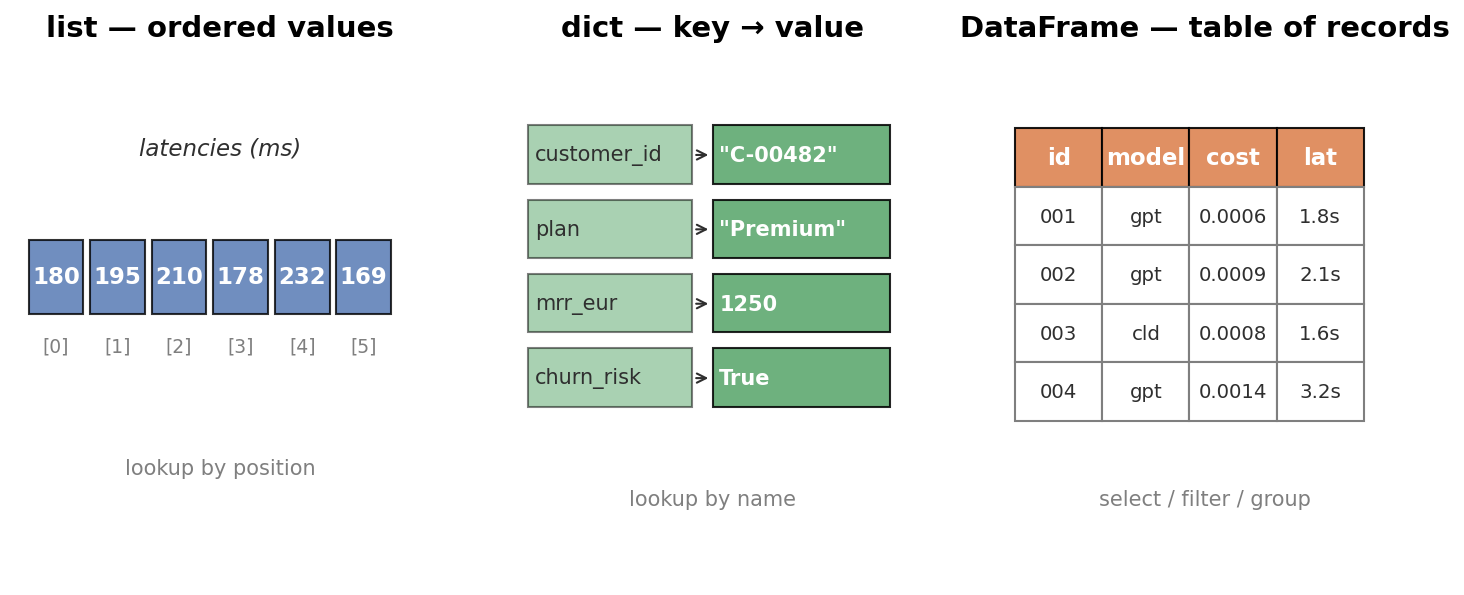
\includegraphics[width=0.97\textwidth,height=0.78\textheight,keepaspectratio]{images/04_list_dict_dataframe.png}
  \end{center}
\end{frame}

\begin{frame}[fragile]{Lists -- ordered, mutable, sliceable}
\begin{lstlisting}
latencies_ms = [180, 195, 210, 178, 232, 169, 204]

latencies_ms[0]       # 180     (first)
latencies_ms[-1]      # 204     (last)
latencies_ms[-3:]     # [169, 204]   wait, that's only 2 -- need [-3:]
latencies_ms[::2]     # every other element
\end{lstlisting}
  \textbf{The single most important pandas-style syntax} -- and it works on plain Python lists, NumPy arrays, and pandas Series unchanged.
\end{frame}

\begin{frame}[fragile]{Dicts -- the JSON / API / LLM shape}
\begin{lstlisting}
api_response = {
    "request_id": "req_9472193",
    "model":      "gpt-4o-mini",
    "usage":      {"input_tokens": 482,
                   "output_tokens": 121,
                   "total_tokens":  603},
    "choices":    [{"message": {"role": "assistant",
                                 "content": "Refunds take 5 business days."}}],
}

reply = api_response["choices"][0]["message"]["content"]
\end{lstlisting}
  Same shape as every web API and every LLM provider's chat format.
\end{frame}

\begin{frame}[fragile]{Defensive parsing -- the production habit}
\begin{lstlisting}
def safe_get(d, path):
    """Walk a nested dict/list. Return None on missing/wrong type."""
    cur = d
    for step in path:
        try:
            cur = cur[step]
        except (KeyError, IndexError, TypeError):
            return None
    return cur

safe_get(resp, ["choices", 0, "message", "content"])  # works
safe_get(resp, ["choices", 5, "message"])              # None, no crash
\end{lstlisting}
  \begin{alertblock}{Rule of thumb}
    Whenever you read data you don't fully control, write the access function
    \emph{defensively once} and use it everywhere.
  \end{alertblock}
\end{frame}

\subsection{Pandas preview}

\begin{frame}[fragile]{A DataFrame is a table you can program against}
\begin{lstlisting}
import pandas as pd

df = pd.DataFrame({
    "request_id": ["req_001", "req_002", "req_003"],
    "model":      ["gpt-4o-mini", "claude-haiku", "gpt-4o-mini"],
    "tokens_in":  [482, 612, 1180],
    "tokens_out": [121, 158, 205],
})

df.shape       # (3, 4)
df["tokens_in"].mean()             # average input tokens
df[df["tokens_in"] > 500]          # filter rows
df.groupby("model")["tokens_in"].sum()
\end{lstlisting}
\end{frame}

\begin{frame}{The five commands you always run first}
  \begin{block}{Inspect any new dataset}
    \begin{itemize}
      \item \texttt{df.head()} -- look at the first few rows
      \item \texttt{df.shape} -- rows $\times$ columns
      \item \texttt{df.dtypes} -- what's a string vs a number
      \item \texttt{df.describe()} -- per-column summary statistics
      \item \texttt{df.info()} -- types + missing-value counts
    \end{itemize}
  \end{block}
  Skipping this step is the most common rookie mistake.
\end{frame}

\begin{frame}[fragile]{Filter, derive, group -- the pandas trio}
\begin{lstlisting}
# Filter: boolean mask
slow = df[df["latency_ms"] > 2000]

# Derive: vectorised arithmetic, no loop
df["cost_usd"] = (df["tokens_in"]  / 1000 * 0.0006 +
                  df["tokens_out"] / 1000 * 0.0024)

# Group: split -> apply -> combine
df.groupby("model").agg(
    n_calls   =("request_id", "count"),
    mean_cost =("cost_usd",   "mean"),
)
\end{lstlisting}
  These three operations cover 80\% of analytical work.
\end{frame}


% ============================================================
\section{Numerical Computing}
% ============================================================

\subsection{Why NumPy}

\begin{frame}{NumPy is the engine under everything}
  \begin{block}{Why it matters for AI work}
    \begin{itemize}
      \item Pandas, scikit-learn, PyTorch, TensorFlow -- all NumPy underneath.
      \item Token counts, costs, embeddings, model weights -- all live in NumPy arrays.
      \item Vectorised arithmetic replaces explicit loops.
    \end{itemize}
  \end{block}
  \vspace{4pt}
  \begin{exampleblock}{The three attributes you check first on any new array}
    \texttt{shape} \quad how many rows $\times$ columns $\times \ldots$ \\
    \texttt{dtype} \quad what kind of number lives in each cell \\
    \texttt{ndim}\phantom{e}\,\quad how many dimensions
  \end{exampleblock}
  Most ML bugs are shape mismatches. \texttt{print(x.shape)} is your first
  debugging move, before anything else.
\end{frame}

\begin{frame}{NumPy is ${\sim}40\times$ faster on real workloads}
  \begin{center}
    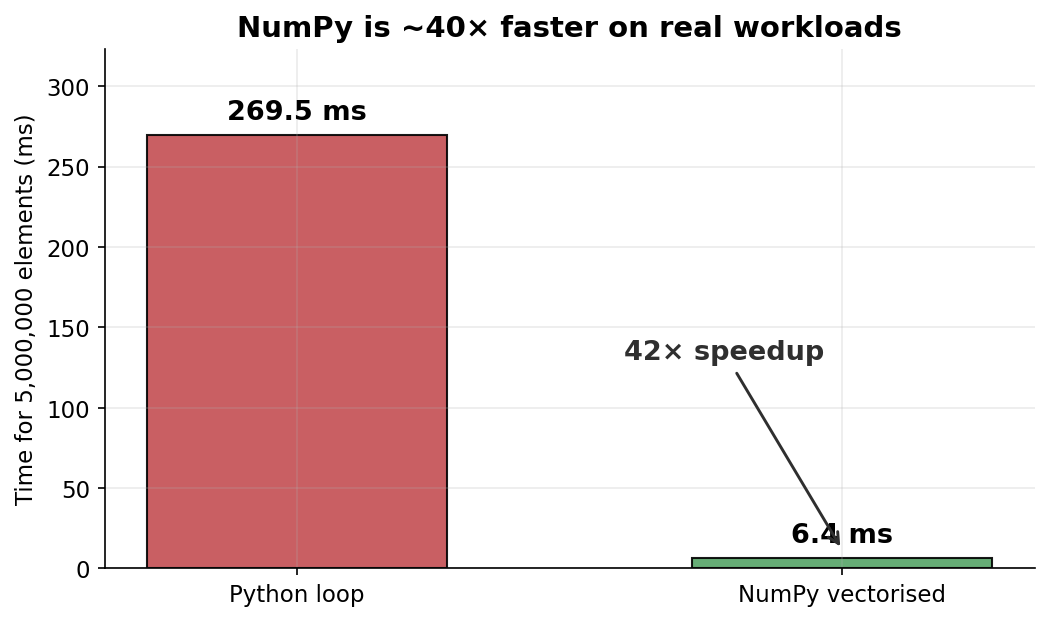
\includegraphics[width=0.80\textwidth,height=0.72\textheight,keepaspectratio]{images/05_numpy_speedup.png}
  \end{center}
\end{frame}

\subsection{Vectorised arithmetic}

\begin{frame}[fragile]{Write the formula, not the loop}
\begin{lstlisting}
import numpy as np

tokens_in  = np.array([480, 720, 305, 610, 815])
tokens_out = np.array([120, 200,  80, 175, 240])

# One vectorised expression -- no Python loop
cost = (tokens_in  / 1000 * 0.0006 +
        tokens_out / 1000 * 0.0024)

cost.sum()           # total spend across the batch
cost.mean()          # average per call
\end{lstlisting}
\end{frame}

\begin{frame}[fragile]{Broadcasting -- the rule that powers everything}
  \begin{block}{The one rule}
    Compare shapes \textbf{from the right}. Dimensions are compatible when they
    are \textbf{equal} or one of them is \textbf{1}.
  \end{block}
  \vspace{6pt}
  \begin{exampleblock}{Example: standardise every column of a feature matrix}
\begin{verbatim}
X_std = (X - X.mean(axis=0)) / X.std(axis=0)
                       # ^^^   shape (3,) - broadcasts across all rows
\end{verbatim}
  \end{exampleblock}
  One line replaces what would otherwise be a nested loop.
\end{frame}

\begin{frame}[fragile]{\texttt{axis=0} vs \texttt{axis=1} -- a mnemonic}
  \begin{block}{The axis that disappears}
    \texttt{X.sum(axis=0)} \emph{eliminates} axis 0 (rows) $\rightarrow$ one value per column.\\
    \texttt{X.sum(axis=1)} \emph{eliminates} axis 1 (columns) $\rightarrow$ one value per row.
  \end{block}
  \vspace{6pt}
  \begin{exampleblock}{Worked example -- per-column mean of a feature matrix}
\begin{verbatim}
X = np.array([[1, 2, 3],          # row 0
              [4, 5, 6],          # row 1
              [7, 8, 9]])         # row 2

X.mean(axis=0)   # [4. 5. 6.]  - one mean per COLUMN  (axis 0 disappears)
X.mean(axis=1)   # [2. 5. 8.]  - one mean per ROW     (axis 1 disappears)
\end{verbatim}
  \end{exampleblock}
  Read ``axis equals $k$'' as ``this axis disappears.''
\end{frame}


% ============================================================
\section{Visualisation}
% ============================================================

\subsection{Pick the right chart}

\begin{frame}{Match the chart to the question}
  \begin{center}
    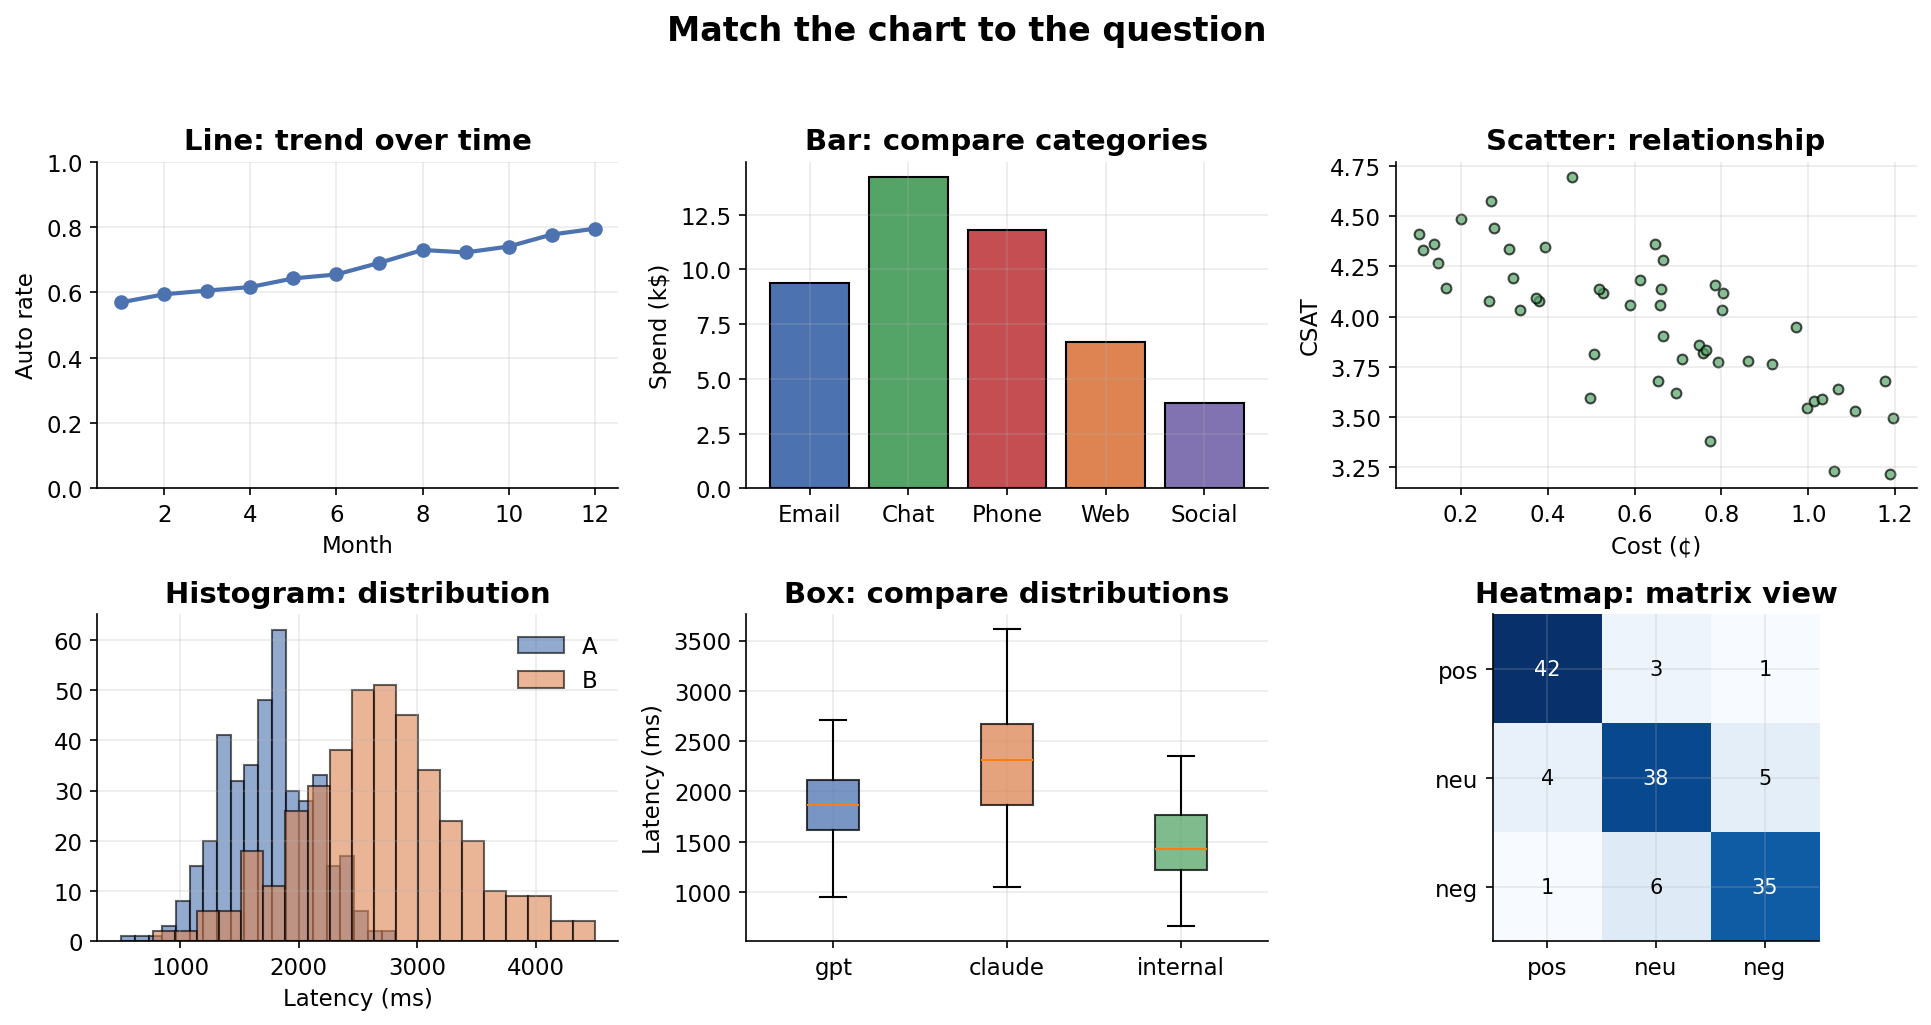
\includegraphics[width=\textwidth,height=0.82\textheight,keepaspectratio]{images/06_chart_gallery.png}
  \end{center}
\end{frame}

\subsection{The Figure / Axes mental model}

\begin{frame}[fragile]{Every chart in 7 lines}
\begin{lstlisting}
fig, ax = plt.subplots(figsize=(8, 4))
ax.plot(x, y, color="#4C72B0", linewidth=2)
ax.set_title("Monthly automation rate")
ax.set_xlabel("Month")
ax.set_ylabel("Automation rate")
plt.tight_layout()
plt.show()
\end{lstlisting}
  \begin{itemize}
    \item \texttt{fig} = the canvas; \texttt{ax} = one plot.
    \item Multiple Axes per Figure $\rightarrow$ dashboards (see the capstone).
    \item Always label axes. A chart without context is a riddle.
  \end{itemize}
\end{frame}

\begin{frame}{Common pitfalls}
  \begin{alertblock}{The five mistakes that always show up}
    \begin{enumerate}
      \item Crowded / overlapping labels $\rightarrow$ call \texttt{plt.tight\_layout()}.
      \item No axis labels $\rightarrow$ always set title + xlabel + ylabel.
      \item Reading off the y-axis $\rightarrow$ annotate bar values directly.
      \item 3-D pie charts $\rightarrow$ almost never use them.
      \item Hard-to-distinguish colours $\rightarrow$ use a small consistent palette.
    \end{enumerate}
  \end{alertblock}
\end{frame}


% ============================================================
\section{Machine Learning}
% ============================================================

\subsection{The workflow}

\begin{frame}{The scikit-learn workflow}
  \begin{center}
    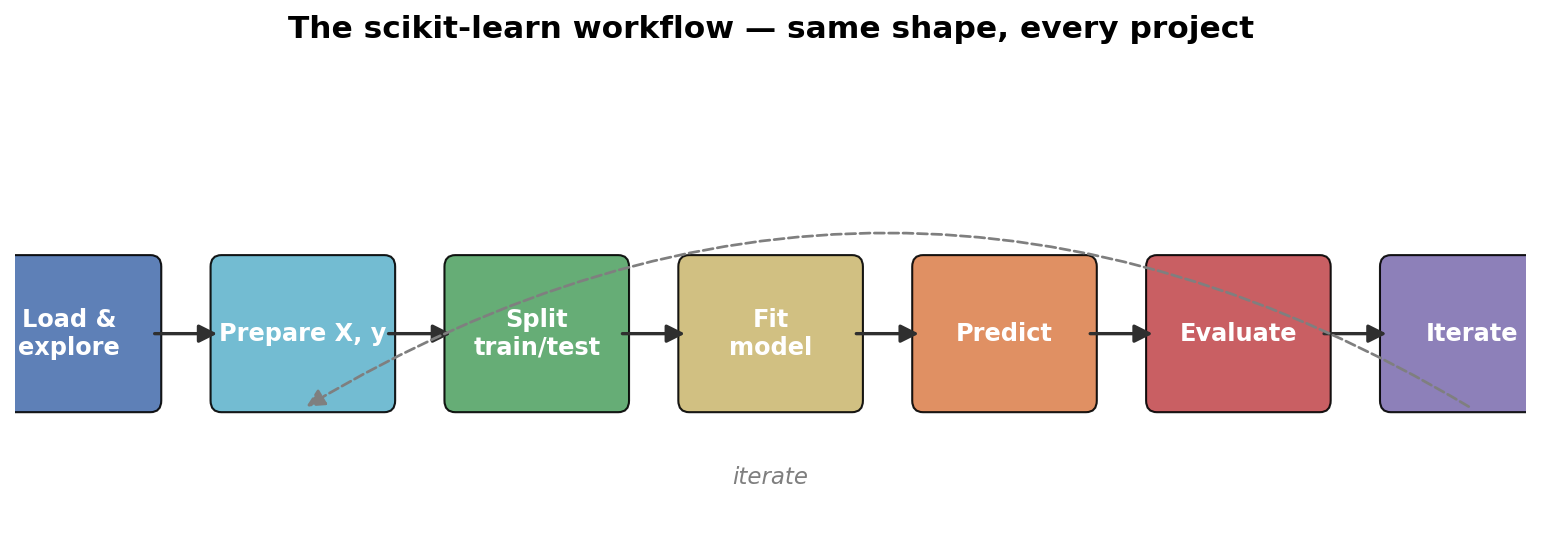
\includegraphics[width=\textwidth,height=0.55\textheight,keepaspectratio]{images/15_ml_workflow.png}
  \end{center}
  \vspace{4pt}
  Every estimator follows the same \texttt{fit / predict / score} contract --
  swapping a logistic regression for a random forest is a one-line change.
\end{frame}

\subsection{Churn prediction}

\begin{frame}{Churn signal is real -- the model can learn it}
  \begin{center}
    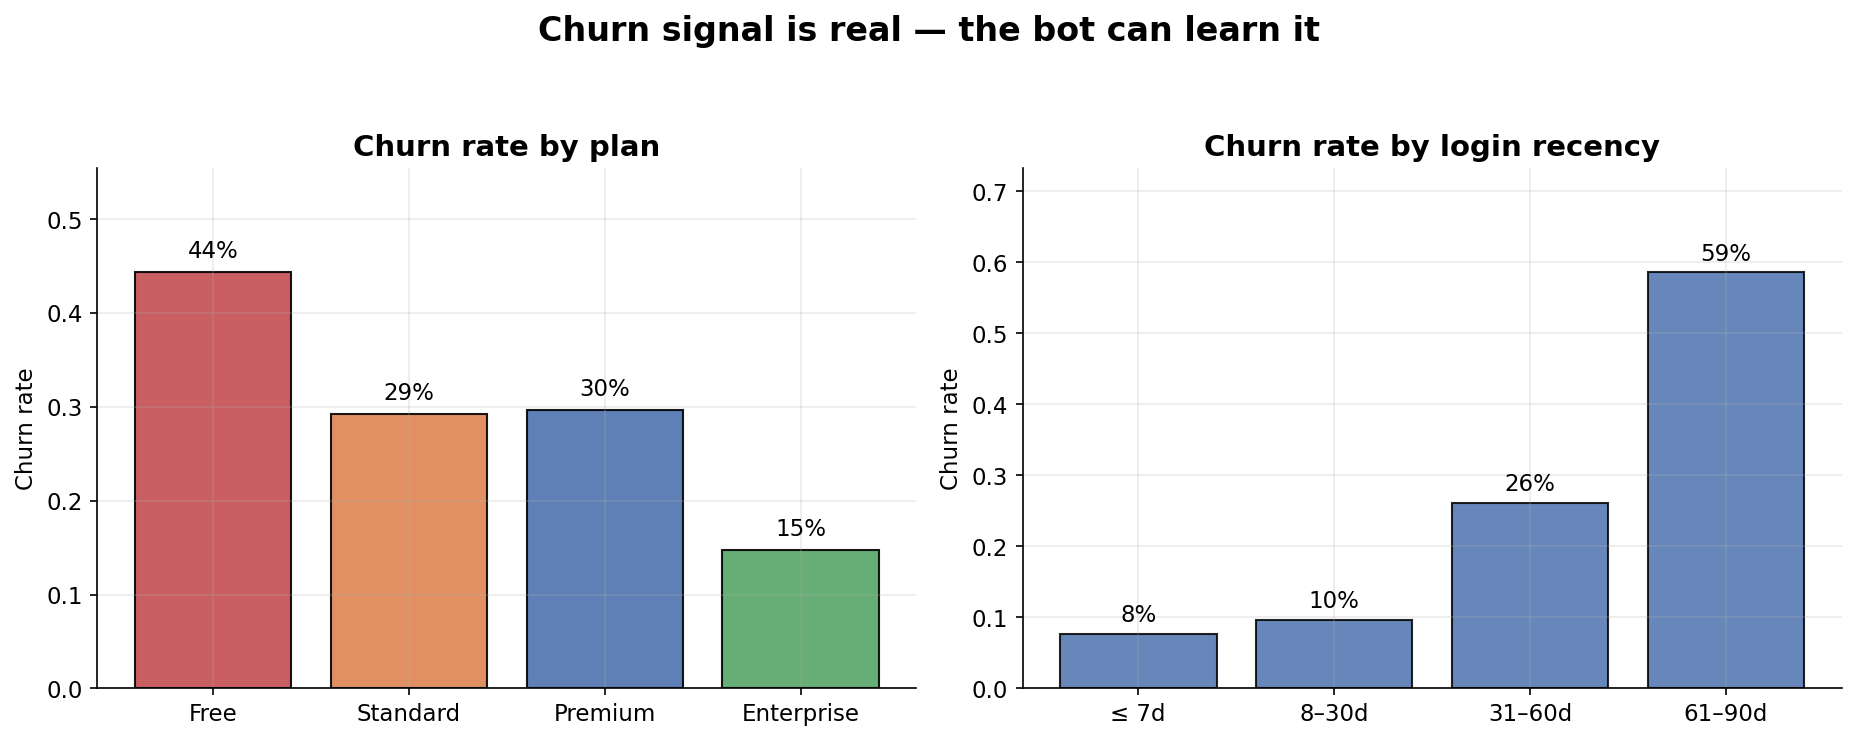
\includegraphics[width=\textwidth,height=0.78\textheight,keepaspectratio]{images/09_churn_by_plan_login.png}
  \end{center}
\end{frame}

\begin{frame}[fragile]{The whole project in eight lines}
\begin{lstlisting}
prep = ColumnTransformer([
    ("num", StandardScaler(), num_cols),
    ("cat", OneHotEncoder(), ["plan"]),
])
pipe = Pipeline([("prep", prep),
                  ("model", RandomForestClassifier(n_estimators=200))])

pipe.fit(X_train, y_train)
print(f"Accuracy: {pipe.score(X_test, y_test):.3f}")  # 0.842
\end{lstlisting}
  \begin{block}{Why the Pipeline matters}
    The scaler and encoder are fit on \emph{training data only} -- never the
    test data. This single discipline prevents \textbf{data leakage}.
  \end{block}
\end{frame}

\begin{frame}{Model results -- the diagnostics that matter}
  \begin{center}
    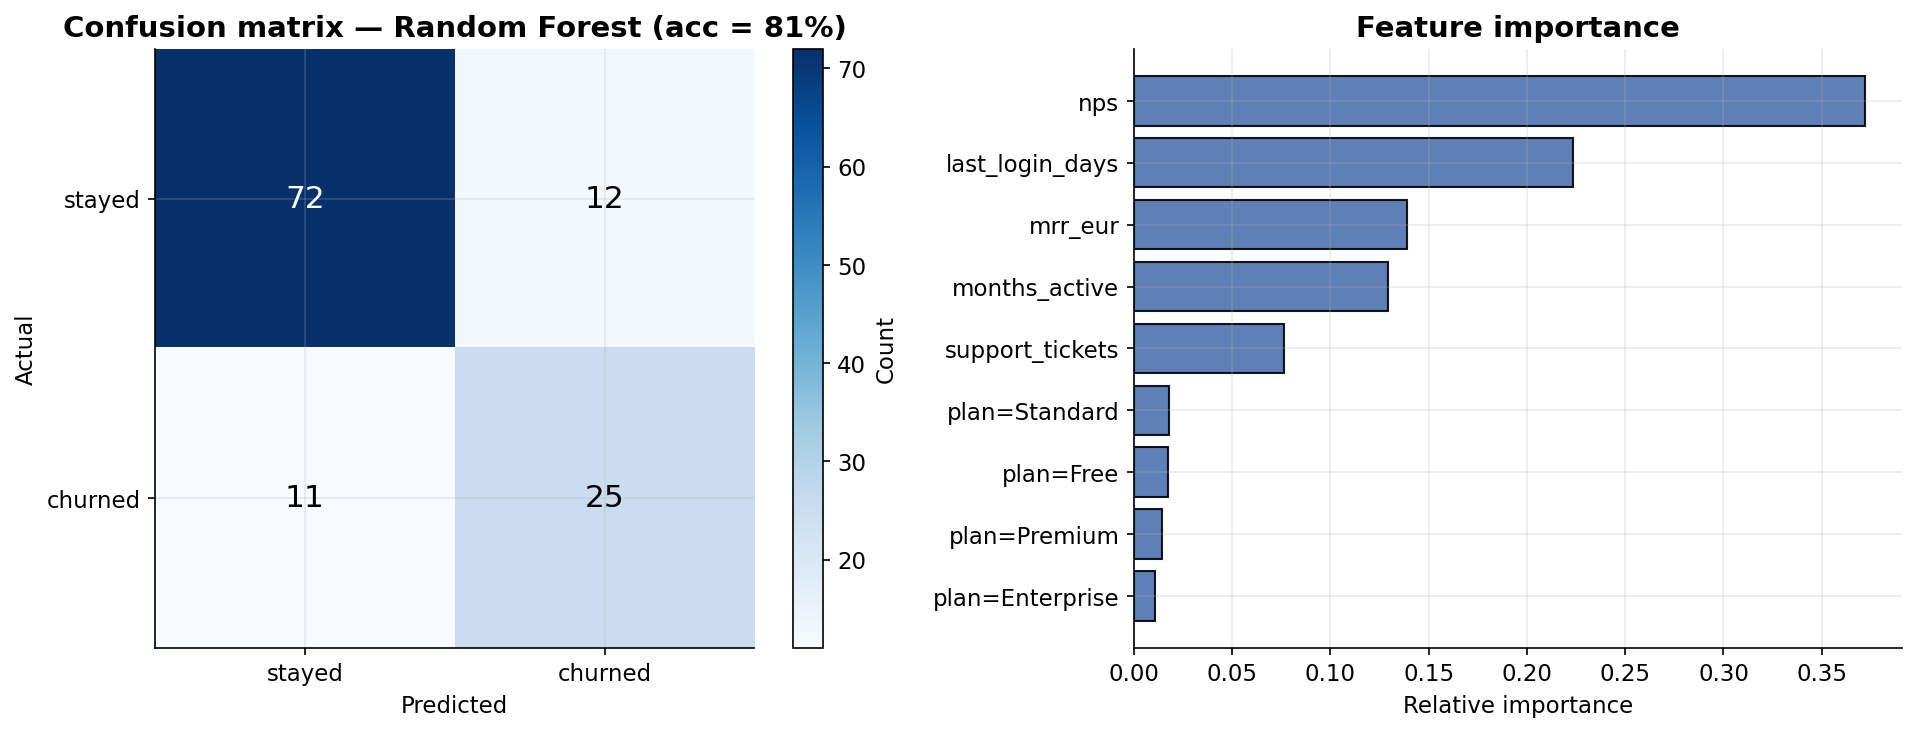
\includegraphics[width=\textwidth,height=0.78\textheight,keepaspectratio]{images/10_churn_model_results.png}
  \end{center}
\end{frame}

\begin{frame}{Beyond accuracy: precision, recall, F1}
  \begin{block}{Which metric matters depends on cost}
    \begin{itemize}
      \item \textbf{High precision} when acting on a flag is expensive (e.g.\ a sales follow-up).
      \item \textbf{High recall} when \emph{missing} a positive is expensive (a churning customer).
      \item \textbf{F1} balances both -- the harmonic mean.
    \end{itemize}
  \end{block}
  \vspace{6pt}
  \begin{alertblock}{Expose probabilities, not just labels}
    \texttt{predict\_proba} returns $P(\text{class})$. A 51\% prediction and a
    95\% prediction are both ``positive'' but tell you very different things
    about how to \emph{act}.
  \end{alertblock}
\end{frame}


% ============================================================
\section{Capstone}
% ============================================================

\subsection{The scenario}

\begin{frame}{The capstone scenario}
  \begin{exampleblock}{The brief}
    You join a SaaS company that deployed an AI support bot at the start of the
    year. The product manager wants \textbf{a single document} that answers:
    \begin{itemize}
      \item Which channels is the bot working in? Which need attention?
      \item Is automation improving across the year?
      \item What's the trade-off between cost and customer satisfaction?
      \item Where should the team invest next?
    \end{itemize}
  \end{exampleblock}
\end{frame}

\begin{frame}{The dataset shape -- 60 rows $\times$ 8 columns}
  Each row is one (channel, month) observation -- same shape as a typical
  operations data-warehouse export.
  \vspace{4pt}
  \begin{exampleblock}{Schema}
    \footnotesize
    \begin{tabular}{ll}
      \toprule
      \textbf{Column} & \textbf{Meaning} \\
      \midrule
      \texttt{channel}, \texttt{month}        & categorical -- 5 channels $\times$ 12 months \\
      \texttt{tickets\_total}, \texttt{tickets\_auto} & ticket counts (total / auto-resolved) \\
      \texttt{automation\_rate}               & auto / total, in $[0, 1]$ \\
      \texttt{latency\_ms}                    & median first-response latency \\
      \texttt{satisfaction}                   & mean CSAT, 1--5 \\
      \texttt{cost\_per\_ticket}              & USD per ticket (LLM + human time) \\
      \bottomrule
    \end{tabular}
  \end{exampleblock}
\end{frame}

\subsection{The dashboard}

\begin{frame}{The deliverable -- one slide, four panels}
  \begin{center}
    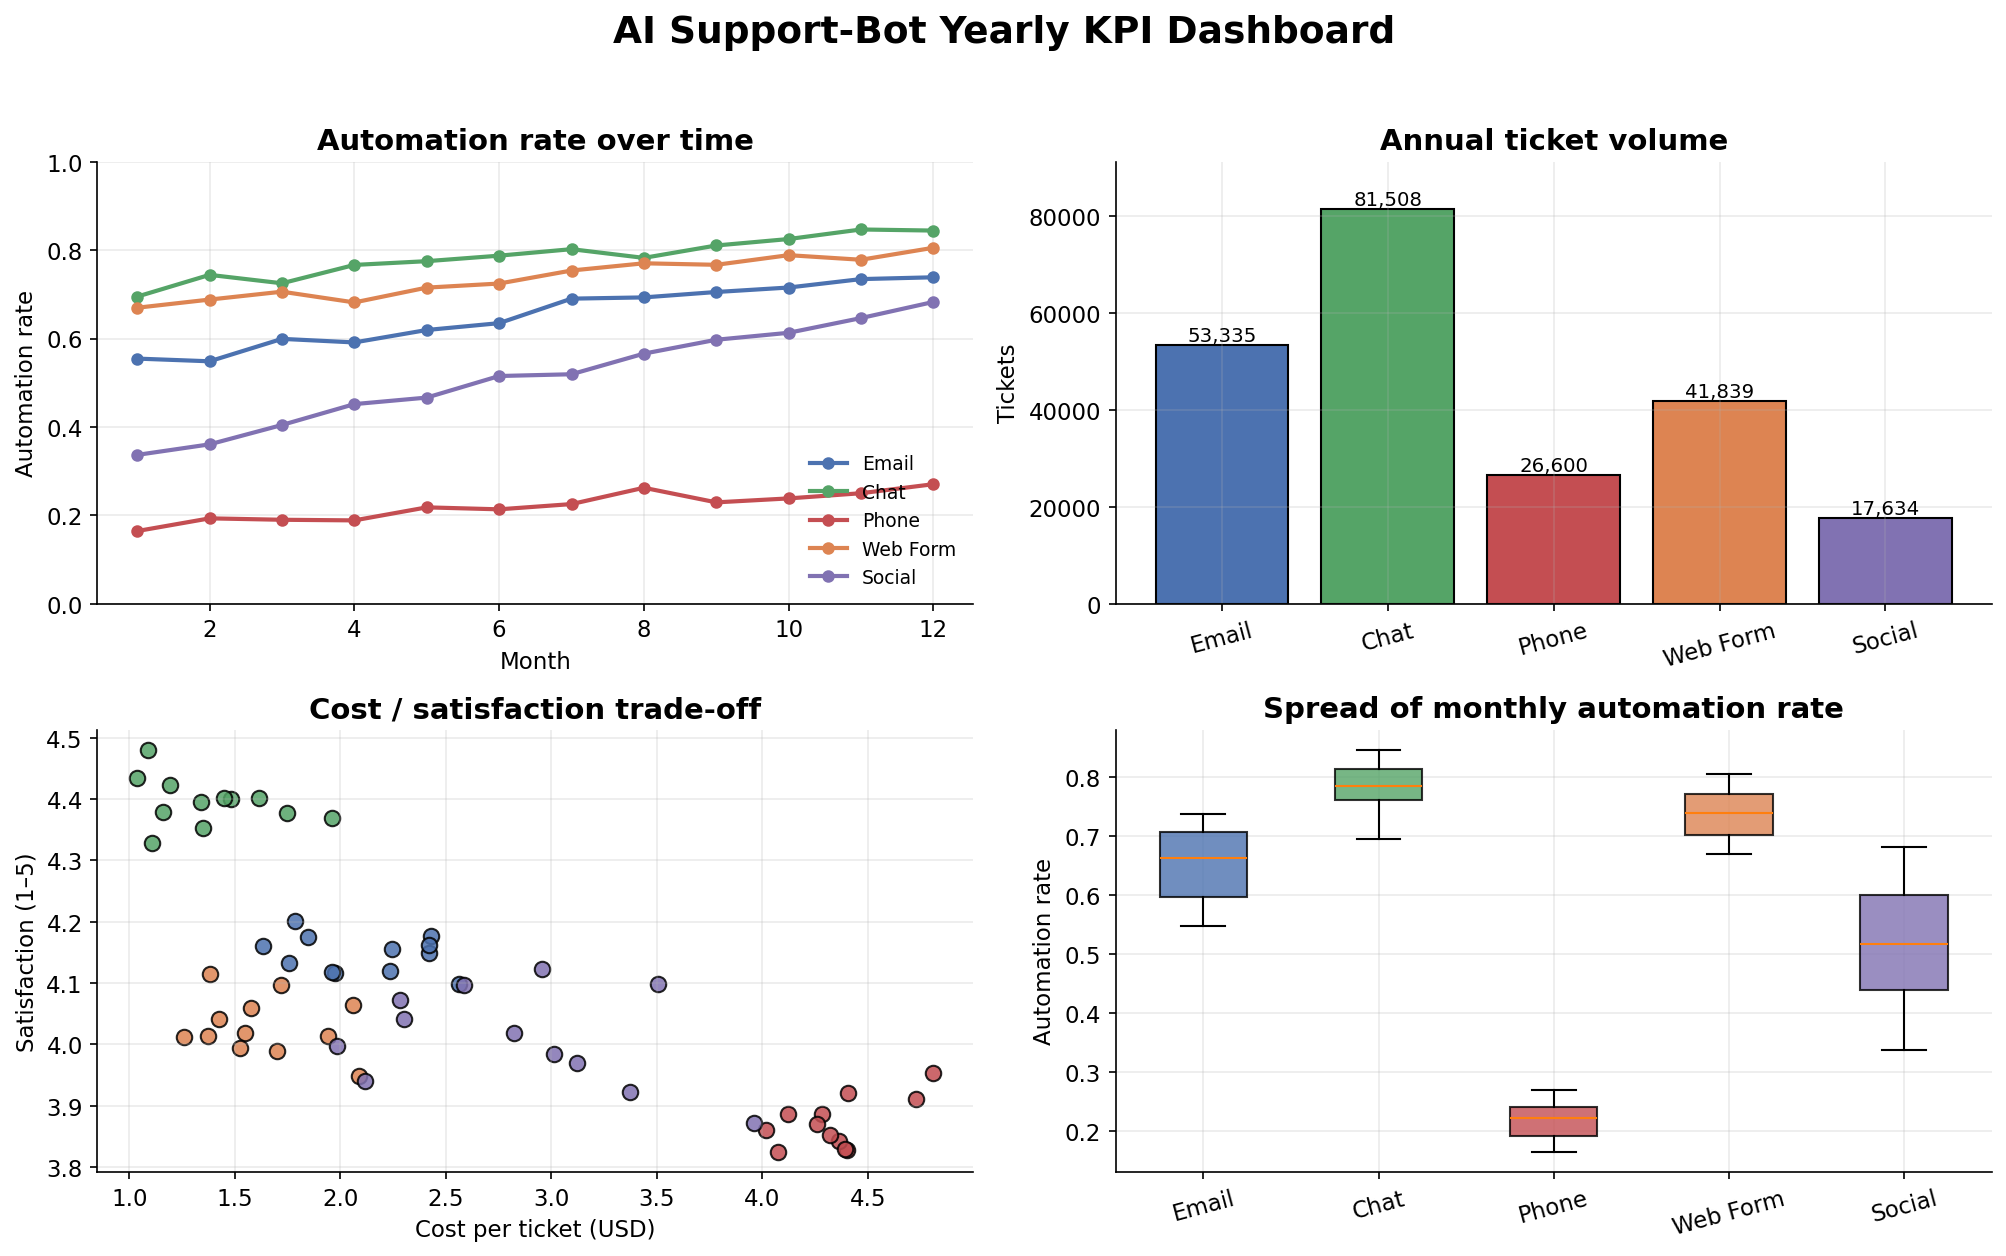
\includegraphics[width=\textwidth,height=0.82\textheight,keepaspectratio]{images/07_capstone_dashboard.png}
  \end{center}
\end{frame}

\begin{frame}{Reading the dashboard}
  \begin{itemize}
    \item \textbf{Top-left.} Every channel trends upward -- Chat and Web Form
          lead; Phone improves slowly from a very low base.
    \item \textbf{Top-right.} Volume is concentrated in Chat and Email --
          where automation gains have the biggest absolute payoff.
    \item \textbf{Bottom-left.} A clear inverse cluster: low cost / high
          satisfaction -- the bot wins. Phone sits in the expensive zone.
    \item \textbf{Bottom-right.} Phone is volatile; Chat is steady. Variance
          matters as much as the mean.
  \end{itemize}
\end{frame}

\subsection{A subtle insight}

\begin{frame}{Simpson's paradox -- the trap to avoid}
  \begin{center}
    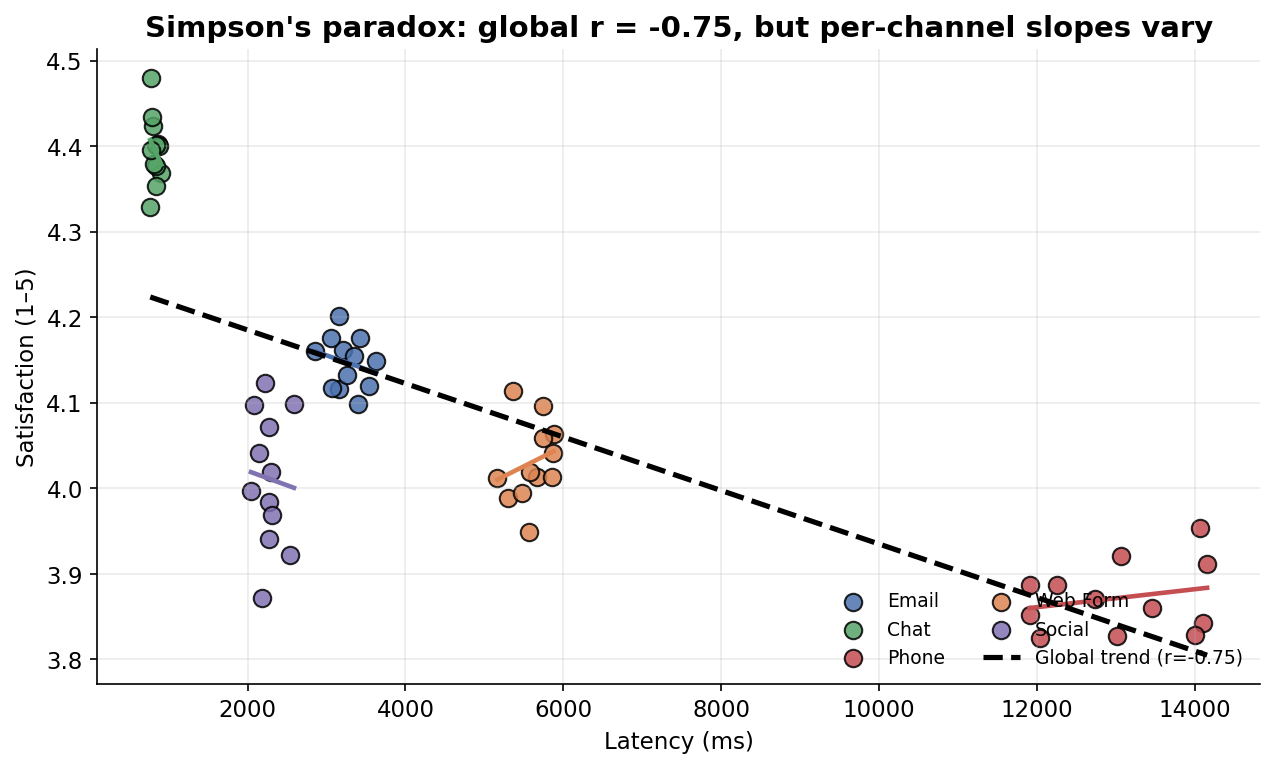
\includegraphics[width=0.95\textwidth,height=0.65\textheight,keepaspectratio]{images/08_simpsons_paradox.png}
  \end{center}
  \begin{alertblock}{The lesson}
    The global correlation is \textbf{misleading}. Always group by category
    before drawing conclusions.
  \end{alertblock}
\end{frame}

\subsection{The executive summary}

\begin{frame}{What you actually deliver}
  \begin{block}{Five bullets a manager can read in 30 seconds}
    \footnotesize
    \begin{enumerate}
      \item Overall automation rate climbed from ${\sim}50\%$ in Q1 to ${\sim}75\%$ in Q4.
      \item Chat and Web Form are the bot's strongest channels and carry $50\%$ of volume.
      \item Phone is the weakest: $<30\%$ automation, highest cost per ticket. Recommendation: route inbound voice to chat.
      \item Latency does \emph{not} drive satisfaction within a channel -- the global negative correlation is a Simpson's paradox artefact.
      \item Social is the breakout: double-digit uplift this year. Invest in Q1 next year.
    \end{enumerate}
  \end{block}
  \vspace{4pt}
  All the code that came before exists to support these five bullets.
\end{frame}


% ============================================================
\section{AI Workflows}
% ============================================================

\subsection{LLMs as function calls}

\begin{frame}[fragile]{An LLM call is just a function call}
  \begin{block}{From your code's perspective}
\begin{verbatim}
response = llm(messages=[...], model="...", temperature=...)
\end{verbatim}
  \end{block}
  \vspace{4pt}
  \begin{exampleblock}{What changes if you adopt this view}
    \begin{itemize}
      \item Typed inputs, structured outputs, retries on failure.
      \item Costs you can measure, latencies you can profile.
      \item Tests you can run, regressions you can catch.
    \end{itemize}
  \end{exampleblock}
  Treat the LLM like any other third-party API -- the engineering hygiene comes free.
\end{frame}

\subsection{Prompt anatomy}

\begin{frame}{Three roles, one call}
  \begin{center}
    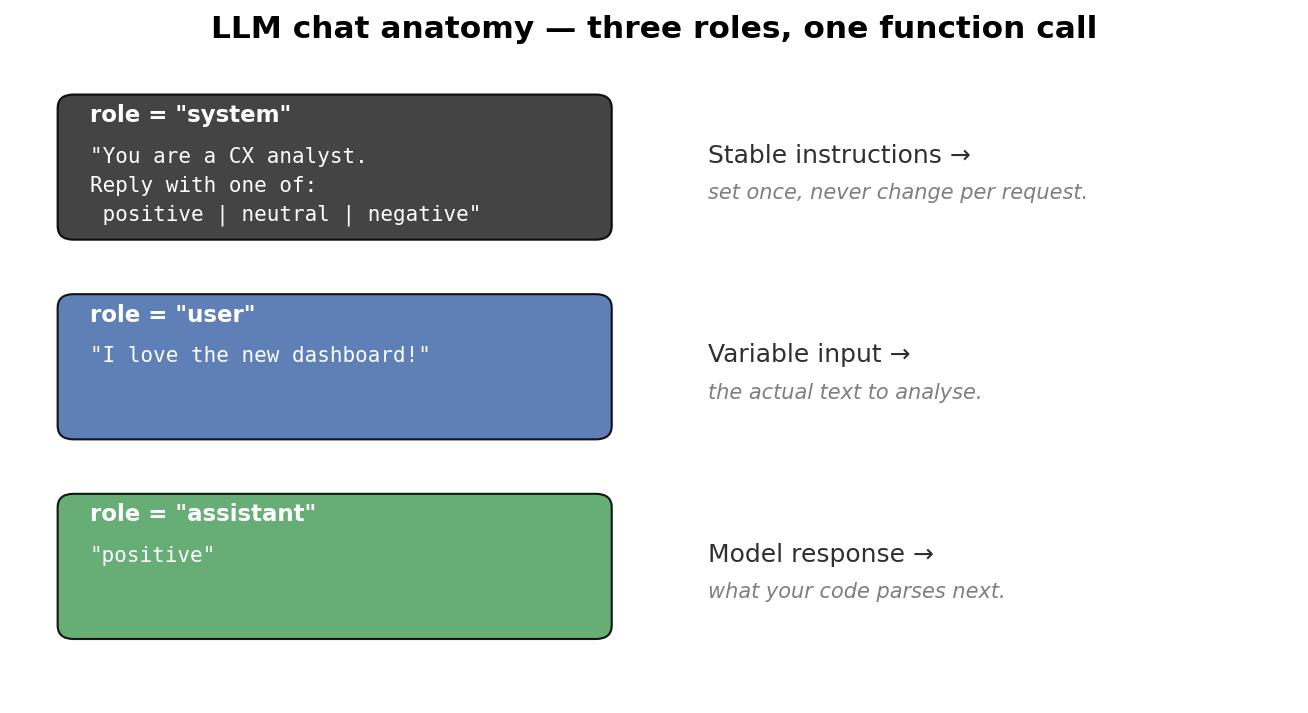
\includegraphics[width=\textwidth,height=0.78\textheight,keepaspectratio]{images/11_prompt_anatomy.png}
  \end{center}
\end{frame}

\begin{frame}{The four prompt patterns}
  \begin{center}
    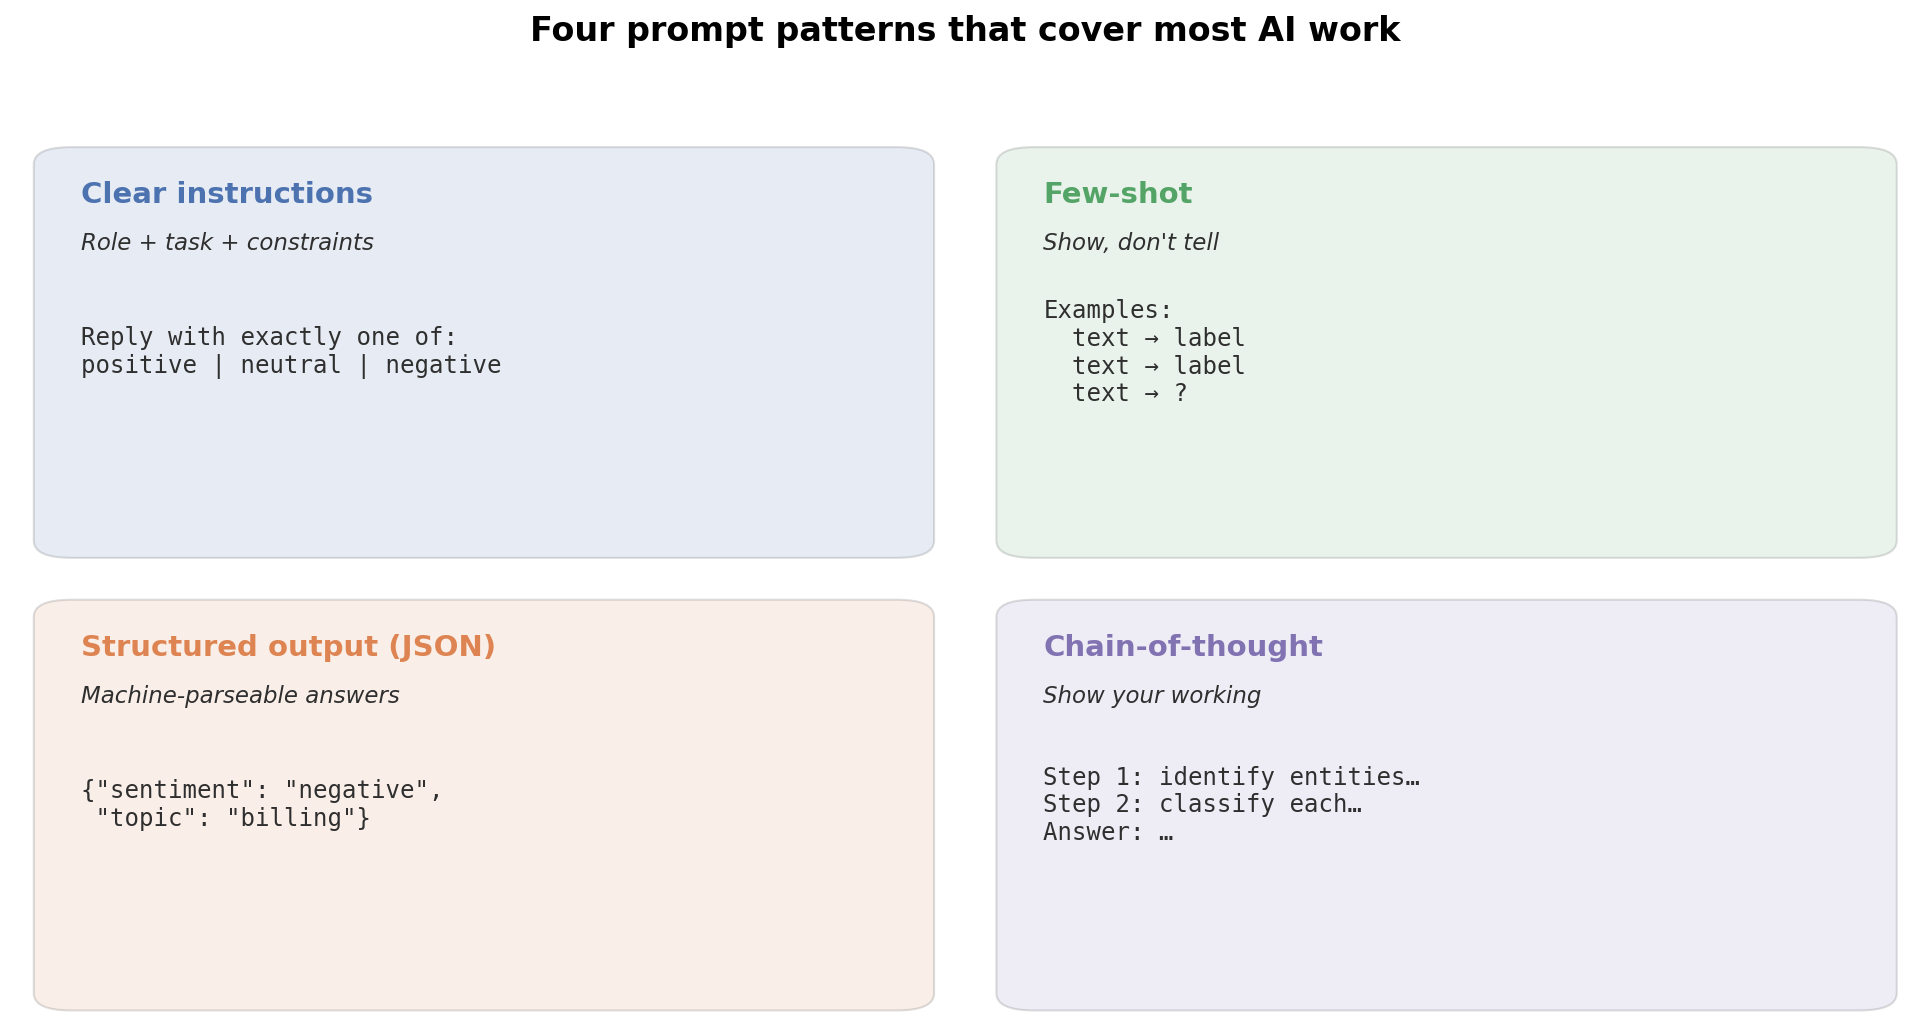
\includegraphics[width=\textwidth,height=0.82\textheight,keepaspectratio]{images/14_prompt_patterns.png}
  \end{center}
\end{frame}

\subsection{Structured output}

\begin{frame}[fragile]{Ask for JSON -- and parse it defensively}
\begin{lstlisting}
SYSTEM = (
    "You analyse customer messages. "
    "Return JSON with keys 'sentiment' (positive/neutral/negative) "
    "and 'topic' (billing/tech/feature/other). Reply with the JSON only."
)

resp = llm.chat(messages=[
    {"role": "system", "content": SYSTEM},
    {"role": "user",   "content": text},
])

try:
    labels = json.loads(resp["text"])
except json.JSONDecodeError:
    labels = {"sentiment": "unknown", "topic": "unknown"}
\end{lstlisting}
  \begin{alertblock}{Always wrap \texttt{json.loads} in \texttt{try/except}}
    Real models occasionally add markdown fences or trailing prose.
  \end{alertblock}
\end{frame}

\subsection{Batch analysis}

\begin{frame}{From messy inbox to actionable categories}
  \begin{center}
    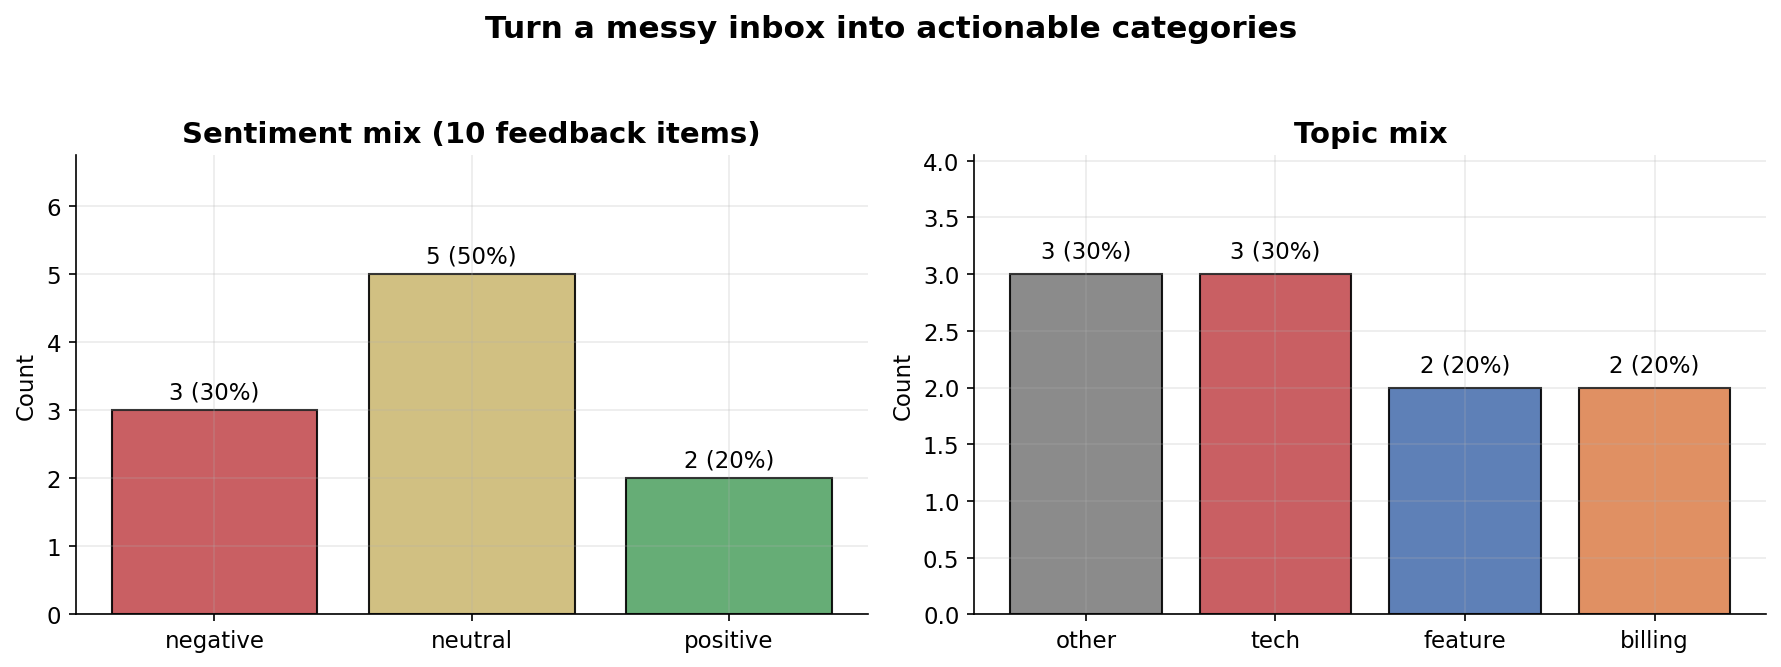
\includegraphics[width=\textwidth,height=0.78\textheight,keepaspectratio]{images/13_batch_analysis.png}
  \end{center}
\end{frame}

\subsection{Retrieval-augmented generation}

\begin{frame}{RAG -- ground the model in your own data}
  \begin{center}
    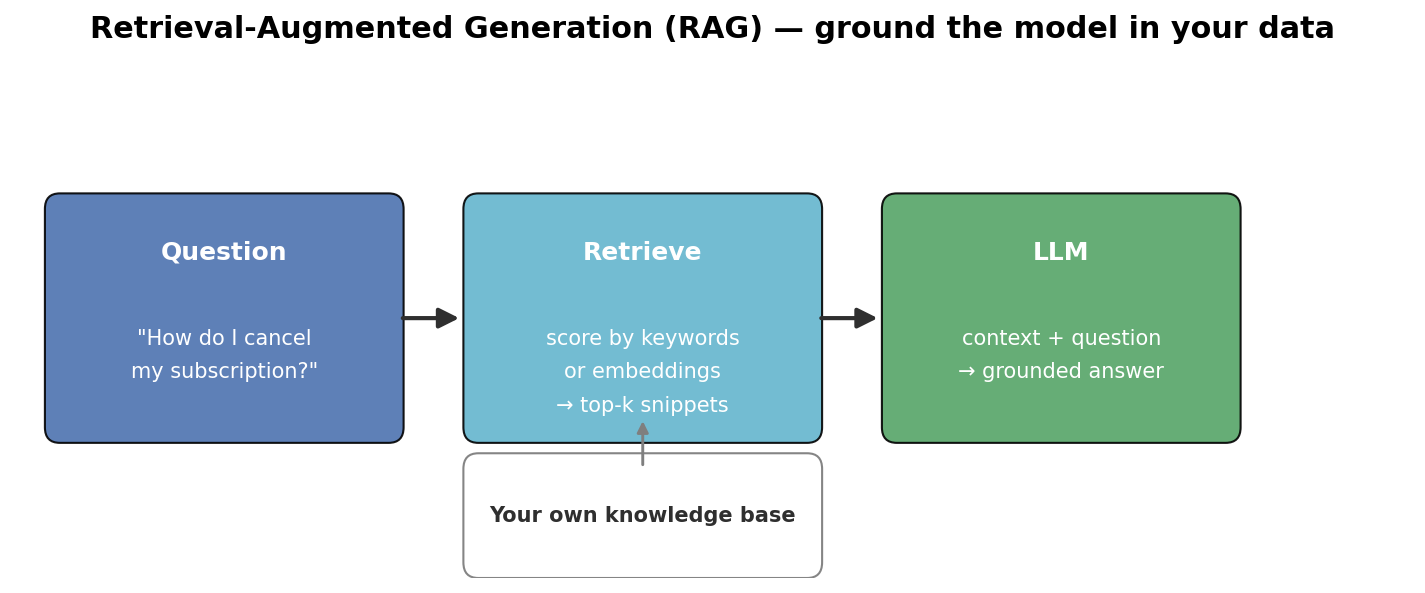
\includegraphics[width=\textwidth,height=0.78\textheight,keepaspectratio]{images/12_rag_pipeline.png}
  \end{center}
\end{frame}

\begin{frame}[fragile]{RAG in roughly 15 lines}
\begin{lstlisting}
def rag_answer(question, docs):
    # 1. Retrieve relevant snippets
    snippets = retrieve(question, docs, k=2)
    context  = "\n\n".join(f"[{name}] {text}" for name, text in snippets)

    # 2. Ask the LLM to answer ONLY from that context
    system = ("You answer the user's question using ONLY the context provided. "
              "If the context does not contain the answer, say so clearly.")
    r = llm.chat(messages=[
        {"role": "system", "content": system},
        {"role": "user",   "content": f"Context:\n{context}\n\nQ: {question}"},
    ])
    return r["text"], snippets
\end{lstlisting}
  Swap keyword matching for vector embeddings to upgrade to production-grade RAG.
\end{frame}

\subsection{The engineer's checklist}

\begin{frame}{Cost, latency, and evaluation -- always}
  \begin{block}{The 30-second regression test}
    Keep a 50--500-example labelled eval set per AI feature. Re-run it on every
    prompt or model change. Three columns are usually enough:
    \texttt{accuracy}, \texttt{latency\_p95}, \texttt{cost\_per\_call}.
  \end{block}
  \vspace{6pt}
  \begin{alertblock}{The single mistake that kills AI projects}
    Shipping a prompt and then \emph{never measuring} how it behaves on real
    inputs. The eval set pays for itself within a week.
  \end{alertblock}
\end{frame}

\subsection{Going live}

\begin{frame}[fragile]{Swap the MockLLM for a real provider}
\begin{lstlisting}
# pip install openai
from openai import OpenAI
client = OpenAI()    # picks up OPENAI_API_KEY from env

def chat(messages, model="gpt-4o-mini", temperature=0.0):
    resp = client.chat.completions.create(
        model=model, messages=messages, temperature=temperature,
    )
    return {"text": resp.choices[0].message.content,
            "tokens_in":  resp.usage.prompt_tokens,
            "tokens_out": resp.usage.completion_tokens}
\end{lstlisting}
  \begin{alertblock}{Never paste API keys into a notebook}
    Use environment variables (\texttt{os.getenv("OPENAI\_API\_KEY")}) or a
    \texttt{.env} file plus \texttt{python-dotenv}.
  \end{alertblock}
\end{frame}


% ============================================================
\section{Wrap-up}
% ============================================================

\subsection{Key takeaways}

\begin{frame}{Eight lessons that travel}
  \begin{enumerate}
    \item \textbf{Functions and pipelines} beat copy-paste -- every time.
    \item \textbf{Defensive parsing} (\texttt{.get(key, default)}, \texttt{try/except}) is non-negotiable for external data.
    \item \textbf{Vectorise} -- write the formula, not the loop.
    \item \textbf{Inspect before you analyse}: \texttt{head / shape / dtypes / describe / info}.
    \item \textbf{Group before correlating} -- Simpson's paradox is real.
    \item \textbf{Test/train split, always.} Probabilities, not just labels.
    \item \textbf{Match the chart to the question.} Annotate the punchline.
    \item \textbf{LLMs are functions.} Structured output makes them composable.
  \end{enumerate}
\end{frame}

\subsection{What to do next}

\begin{frame}{Where to go from here}
  \begin{block}{Natural extensions of this course}
    \begin{itemize}
      \item Embeddings + vector stores -- upgrade keyword retrieval to semantic search.
      \item Tool / function calling -- let the LLM call your functions.
      \item Agents -- multi-step reasoning loops that plan, act, observe.
      \item Evaluation frameworks -- automated scoring beyond exact match.
    \end{itemize}
  \end{block}
  \vspace{6pt}
  You now have the Python fluency and the AI-engineering vocabulary to read the
  next tutorial and \emph{follow what is going on} -- which is more than half
  the battle.
\end{frame}

\begin{frame}
  \begin{center}
    {\Huge\bfseries Happy coding.}\\[8pt]
    \large Open a notebook. Edit one number. Re-run. Iterate.
  \end{center}
\end{frame}


\end{document}
